\subsection{Constrained Random Walk Algorithm}
\label{crw_alg}
\begin{algorithm}[ht]
\caption{Constrained Random Walk (CRW)}
\label{alg:crw}
\begin{algorithmic}[1]
\STATE \textbf{Input:} KG executor, seed set $\mathcal{E}$, predicate set $\mathcal{P}$, target size $N$
\STATE \textbf{Output:} trajectory set $\mathcal{D}_{\text{crw}}$
\STATE $\mathcal{D}_{\text{crw}}\leftarrow\emptyset$
\WHILE{$|\mathcal{D}_{\text{crw}}| < N$}
  \STATE Sample seed entity $e_0 \sim \mathcal{E}$ and hop length $L$
  \STATE Initialize partial path $\pi\leftarrow[e_0]$
  \FOR{$t=0$ to $L-1$}
    \STATE Retrieve outgoing candidate relations of $e_t$, then keep $\mathcal{R}_t=\mathcal{R}(e_t)\cap\mathcal{P}$
    \IF{$\mathcal{R}_t=\emptyset$}
      \STATE \textbf{break}
    \ENDIF
    \STATE Sample relation $r_t\sim \mathcal{R}_t$, then sample next node $e_{t+1}\sim \mathcal{N}(e_t,r_t)$
    \STATE Append $(r_t,e_{t+1})$ to $\pi$
  \ENDFOR
  \IF{$\pi$ is valid}
    \STATE Add $\pi$ to $\mathcal{D}_{\text{crw}}$
  \ENDIF
\ENDWHILE
\STATE \textbf{return} $\mathcal{D}_{\text{crw}}$
\end{algorithmic}
\end{algorithm}



\subsection{Semantic Contamination Analysis}
\label{app:contamination}

To preclude knowledge leakage in GraphSynth-15k, we compute the maximum cosine similarity between each synthetic question and all test questions across WebQSP, CWQ, and GrailQA using BGE-M3~\citep{chen2024m3}.
At a strict threshold of 0.85, only 2.57\% of GraphSynth questions exhibit high semantic overlap with any test question, and all flagged samples are excluded from the final training corpus.
The elevated overlap rate against CWQ at threshold 0.80 (23.30\%) reflects expected domain proximity rather than leakage, as CWQ encompasses the most diverse relations and broadest domain coverage among the three benchmarks.
Table~\ref{tab:contamination} and Figure~\ref{fig:contamination_cdf} present the full results.

\begin{table}[h]
\centering
\small
\caption{Contamination rates at three similarity thresholds (BGE-M3).}
\label{tab:contamination}
\begin{tabular}{lcccc}
\toprule
\textbf{Threshold} & \textbf{Overall} & \textbf{CWQ} & \textbf{WebQSP} & \textbf{GrailQA} \\
\midrule
0.80 & 25.97\% (3960) & 23.30\% (3553) & 5.27\% (804) & 2.67\% (407) \\
0.85 &  2.57\% (392)  &  2.13\% (325)  & 0.56\% (85)  & 0.09\% (13)  \\
0.90 &  0.15\% (23)   &  0.12\% (18)   & 0.03\% (4)   & 0.01\% (1)   \\
\bottomrule
\end{tabular}
\end{table}

\begin{figure*}[t]
    \centering
    \begin{subfigure}[b]{0.22\linewidth}
        \centering
        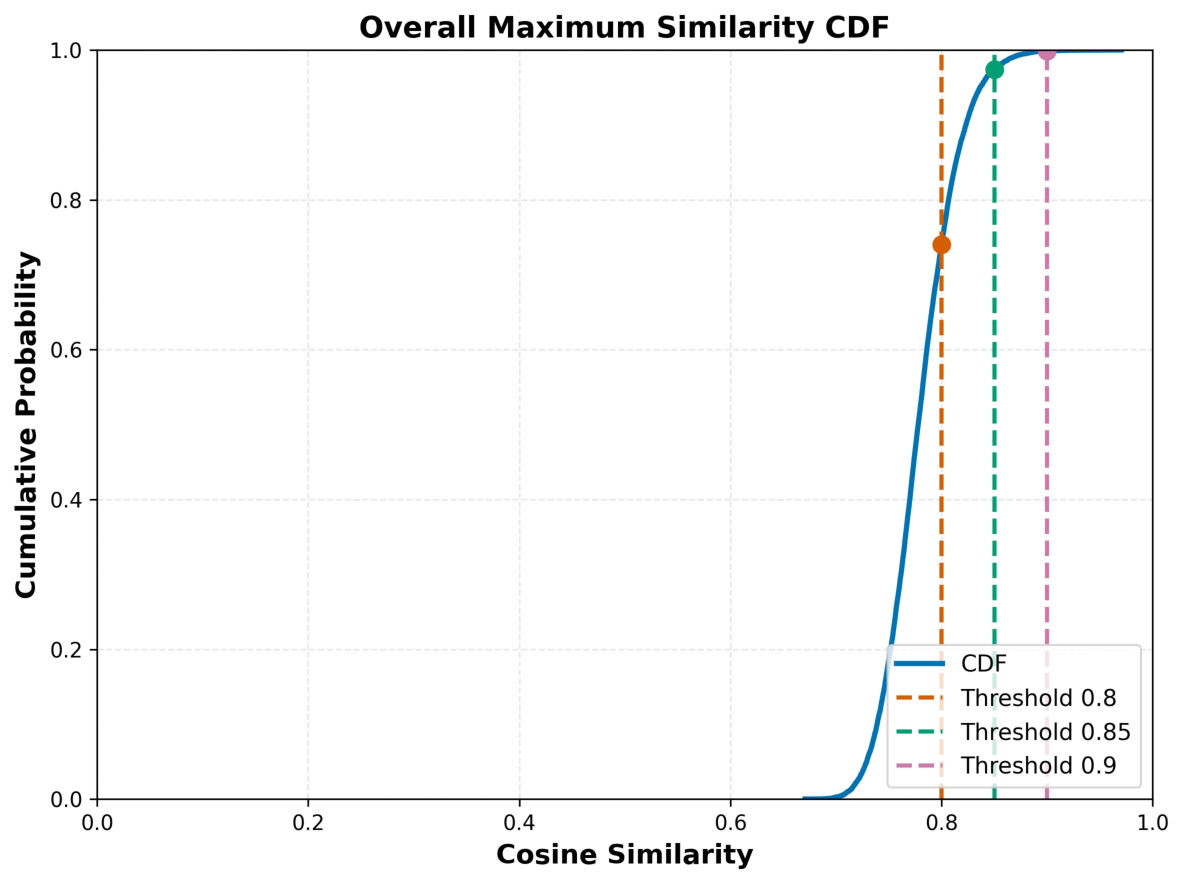
\includegraphics[width=\linewidth]{figures/contamination_cdf.pdf}
        \caption{CDF of maximum semantic similarity.}
        \label{fig:contamination_cdf}
    \end{subfigure}
    \hfill
    \begin{subfigure}[b]{0.74\linewidth}
        \centering
        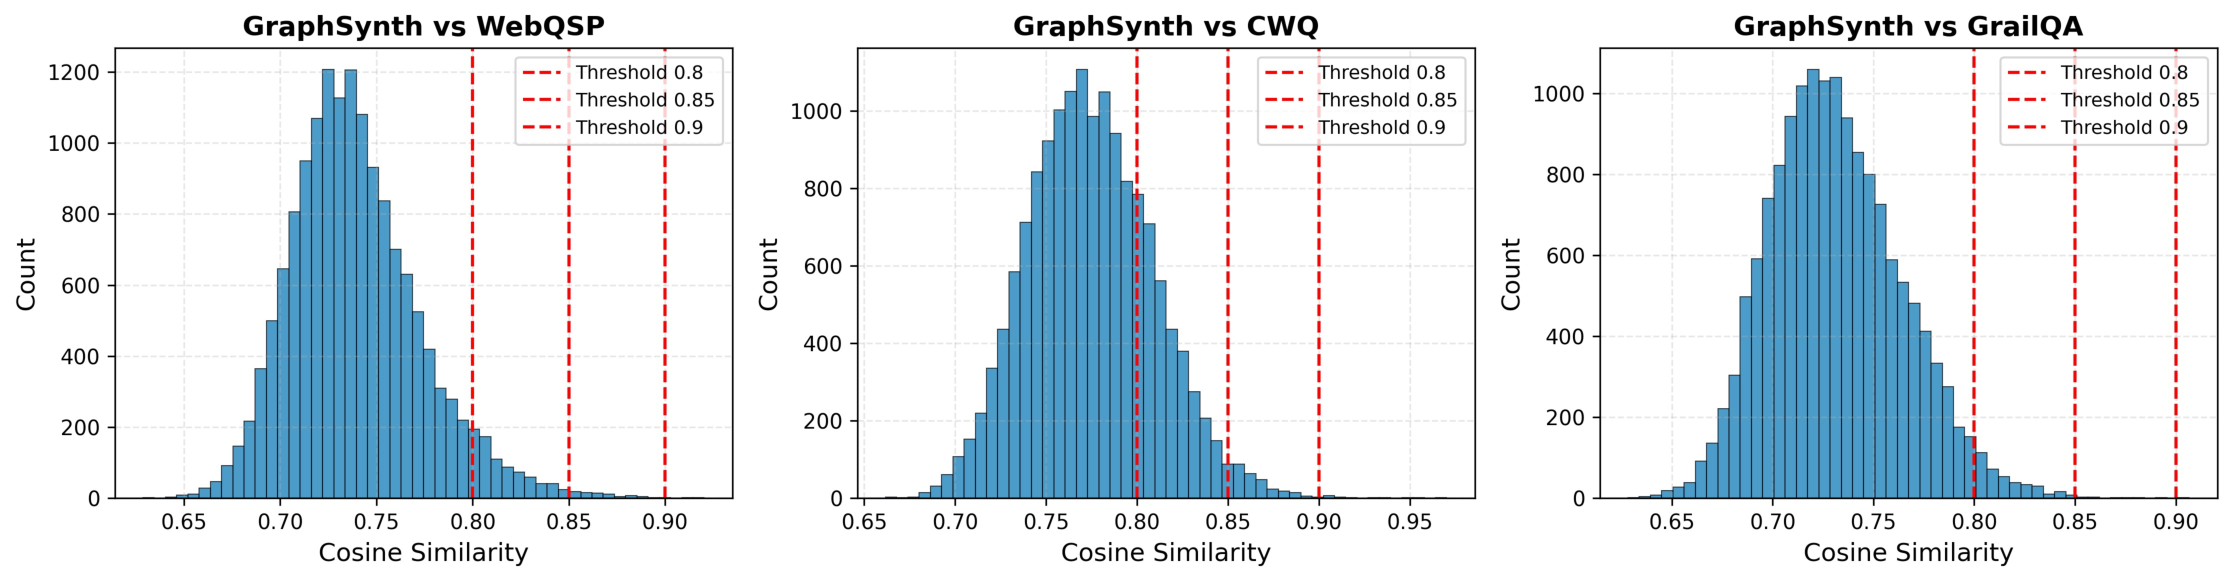
\includegraphics[width=\linewidth]{figures/contamination_histogram.pdf}
        \caption{Semantic cosine similarity distribution on each benchmark.}
        \label{fig:contamination_hist}
    \end{subfigure}
    \caption{Data contamination analysis between GraphSynth and downstream benchmarks.}
    \label{fig:contamination}
    \vspace{-14pt}
\end{figure*}


\subsection{Statistics of GraphSynth}
\label{app:stat_graphsynth}

\begin{table}[htbp]
  \centering
  \small
  \setlength{\tabcolsep}{6pt}
  \caption{Structure distribution of the GraphSynth-15k dataset.}
  \label{tab:graphtrails-e-type}
  \begin{tabular}{l cccc c c}
    \toprule
    \multirow{2}{*}{\textbf{Structure Type}} & \multicolumn{4}{c}{\textbf{Composition}} & \textbf{Conjunction} & \multirow{2}{*}{\textbf{Total}} \\
    \cmidrule(lr){2-5} \cmidrule(lr){6-6}
    & \textbf{2-hop} & \textbf{3-hop} & \textbf{4-hop} & \textbf{5-hop} & \textbf{2I} & \\
    \midrule
    \textbf{Count} & 1,982 & 4,920 & 1,778 & 576 & 5,599 & 14,855 \\
    \textbf{Ratio (\%)} & 13.34 & 33.12 & 11.97 & 3.88 & 37.69 & 100.00 \\
    \bottomrule
  \end{tabular}
\end{table}

\begin{wrapfigure}{r}{0.40\textwidth}
    \vspace{-12pt}
    \centering
    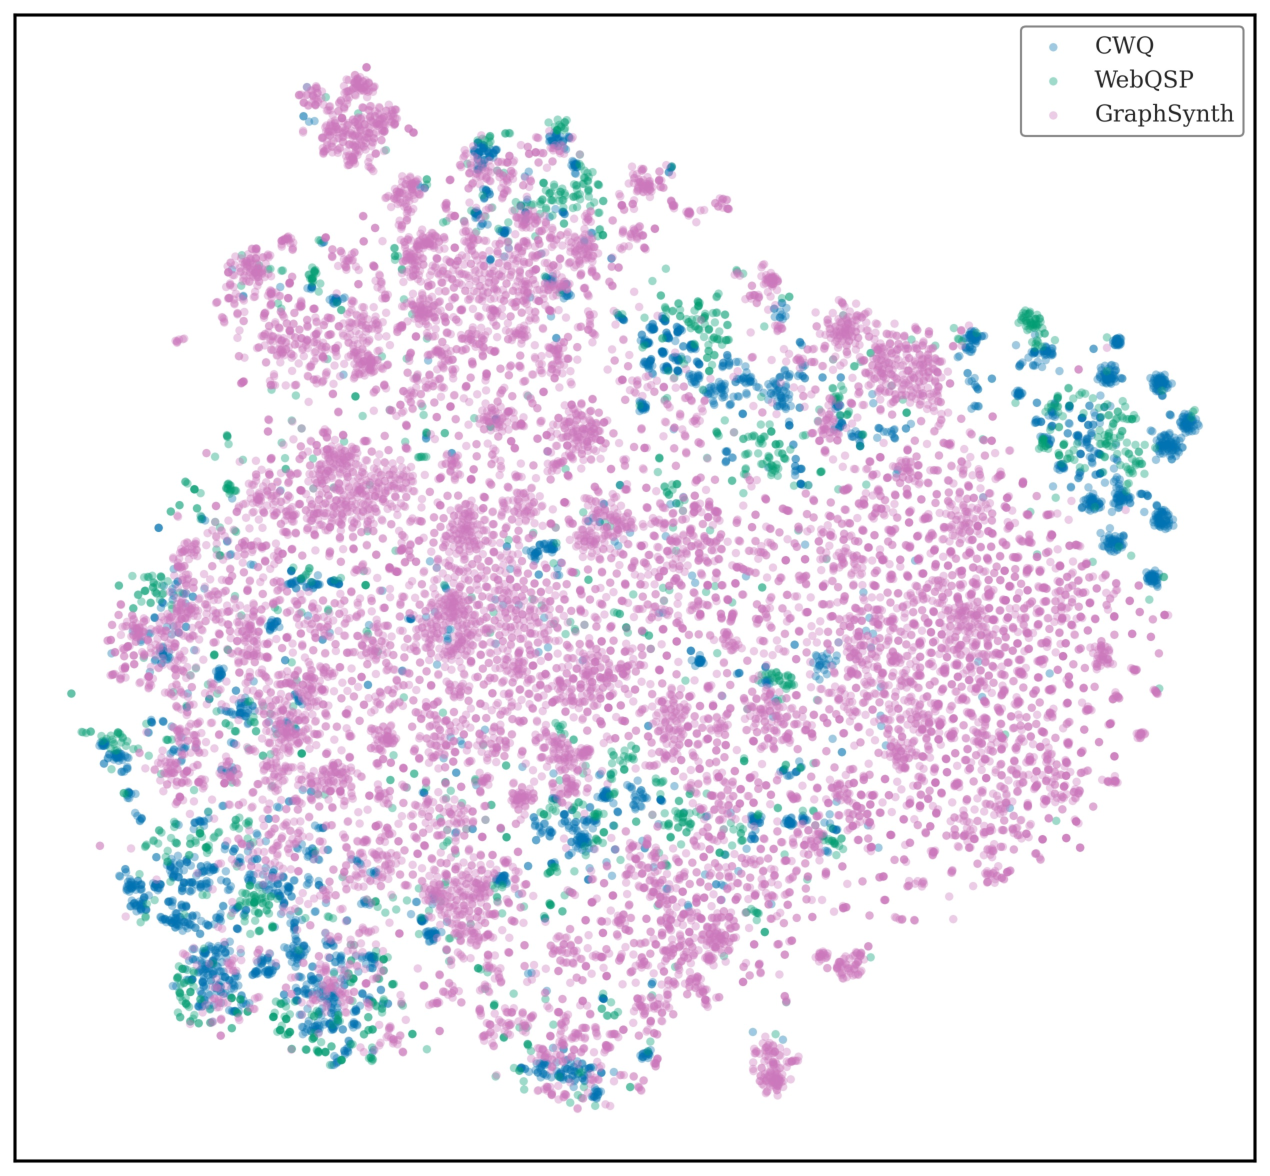
\includegraphics[width=\linewidth]{figures/tsne.pdf}
    \caption{t-SNE visualization of GraphSynth, CWQ, and WebQSP question embeddings, illustrating the broad semantic coverage of the synthesized corpus.}
    \label{fig:tsne}
    \vspace{-10pt}
\end{wrapfigure}

In this section, we characterize GraphSynth-15k along two dimensions to validate its suitability as a training corpus.
Structurally, as summarized in Table~\ref{tab:graphtrails-e-type}, GraphSynth spans five reasoning structure types, covering multi-hop compositions (2- to 5-hop) and conjunctions (2I), with 3-hop and 2I patterns accounting for over 70\% of samples while longer chains ensure exposure to complex reasoning patterns.
Semantically, the synthesized questions are grounded in Freebase relations drawn from diverse topical domains, achieving broad coverage of real-world entity types and relation schemas.
As visualized in Figure~\ref{fig:tsne}, the question embeddings of GraphSynth spread across a wide region of the semantic space, overlapping substantially with both CWQ and WebQSP without concentrating around any single benchmark cluster, confirming that the corpus is neither narrowly specialized nor artificially constrained to a particular domain.
Together, these properties ensure that GraphSynth provides structurally and semantically diverse supervision for Stage 1 training.


